\documentclass[10pt,conference,compsocconf]{IEEEtran}

\usepackage{hyperref}
\usepackage{graphicx}	% For figure environment
\usepackage{subfigure} 

\begin{document}
\title{\#70 - Higgs Boson's Challenge}

\author{
  Joachim Huet, Audrey Loeffel \& Yalan Yiue\\
  \textit{PCML Project 1, 2016}
}

\maketitle

\begin{abstract}
The Higgs boson is an recently discovered particle which explains the causation of mass. In this project, we apply machine learning techniques taught in PCML classes in order to develop a process of rediscovering this particle. In the report, we will present our methodology and results for the Higgs Boson's Challenge that took place in the PCML class at EPFL.
\end{abstract}

\section{Introduction}

In this project, our goal was to build a prediction model based on a dataset provided by the {CERN}. We tried several machine learning methods and optimized their parameters in order to obtain the best predictions. Those methods include least square, logistic regression and ridge regression. 

\section{Methodology}
\label{sec:structure-paper}

For each model we follow a pipeline of computations: clean-up, normalization, improving data set basis and finally building the model. Each step is described below.

\subsection{Pre-computational analysis}

The data are composed of $N = 30$ features and $D = 250000$ samples.
After analysing the data, we figured out that a lot of data were missing and were represented by the value $-999$. 
We also observed that the data weren't centered around 0, that means we needed to standardize them before building any models.
We ignored the $-999$ values during the standardization otherwise they acted like a bias in the mean and the standard deviation computations.

We also tried to ignore features that have more then $50\%$ of null values.

\subsection{Models comparisons}
We implemented multiple models to predict the output of the testing data set
and compare them between each other in order to find the best model.

All methods are presented below.

\subsubsection{Least Squares}
At first we trained a baseline model with the original data set. We didn't do any normalization or optimization. We obtained a score of $0.64$.
On the top of this model we tried to improve our data sets by normalizing it and add a polynomial basis. With a polynomial basis of degree two we reached a score of 0.76. For the implementation, we tried linear regression with both gradient decent and stochastic gradient decent. The data size in this project is acceptable for both regression. 

\subsubsection{Ridge Regression}

The next step was to apply the ridge regression with all feature and without any feature transformation. We obtained a testing error of $0.340048$ as our baseline.

Then we tried some polynomial basis of different degrees. The table below shows the different errors we obtained. 

\begin{figure}[!h]
\center
\subfigure[Degree 2]{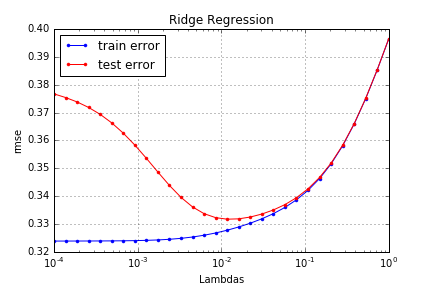
\includegraphics[width=2.3in]{figures/cross_validation_ridge_d2.png} \label{fig:degree2}}
\subfigure[Degree 3]{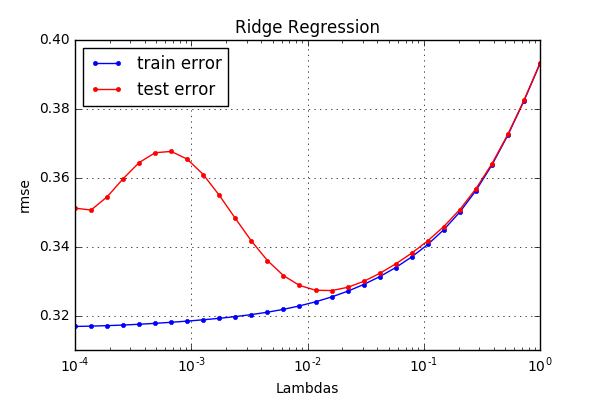
\includegraphics[width=2.3in]{figures/cross_validation_ridge_d3.png} \label{fig:degree3}}
\subfigure[Degree 4]{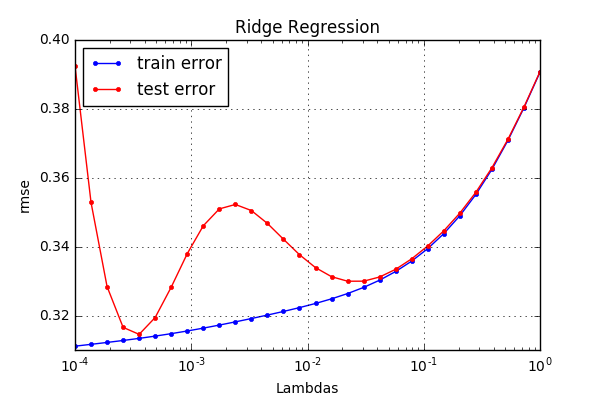
\includegraphics[width=2.3in]{figures/cross_validation_ridge_d4.png} \label{fig:degree4}}
\subfigure[Degree 5]{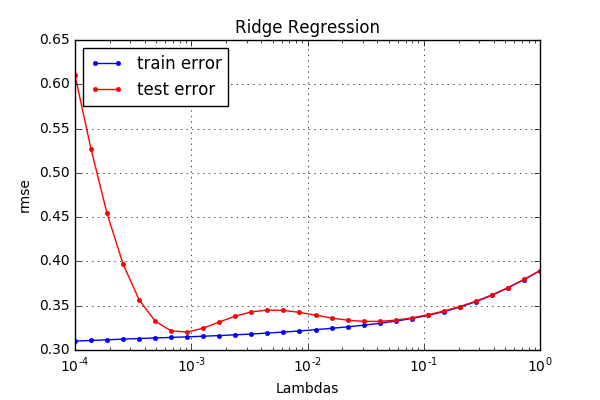
\includegraphics[width=2.3in]{figures/cross_validation_ridge_d5.png} \label{fig:degree5}}
\caption{Ridge Regression with polynomial basis}
\end{figure}


\begin{table}[!h]
\begin{center}
\begin{tabular}{|c||c|c|c|c|}
    \hline
    Method & lambda & Training error & Test error  \\
    \hline\hline
    Baseline & 0.0001 & $0.339968$ & $0.340048$ \\
    \hline
    Polynomial of degree 2& $0.0117210$ &$0.32780$ & $0.33175$ \\
    \hline
    Polynomial of degree 3& $0.0001$ &$0.316836$&$0.351177$ \\
    \hline
    Polynomial of degree 4& $0.00035$ &$0.31337$&$0.314539$ \\
    \hline
    Polynomial of degree 5& $0.00067$ &$0.31421$&$0.32155$ \\
    \hline
\end{tabular}
\caption{RMSE with Ridge Regression}
\label{table:ridgeTable}
\end{center}
\end{table}

We obtained our best model with a polynomial basis of degree 4. As we can see on the table above, the model tends to overfit with a degree greater than two.

\subsubsection{Logistic Regression}

In the case of logistic regression, we implement with regularized logistic regression, and we can thus benefit from the lambda term which avoid the model being too complex. The model tends to diverge when the gamma parameter is too large. In the other hand, if the gamma is too small, the weights are almost unaffected by the gradient during the iterations. The point is to find the best gamma parameter that fit the data, otherwise the predictions are inaccurate.

\begin{figure}[!h]
    \centering
    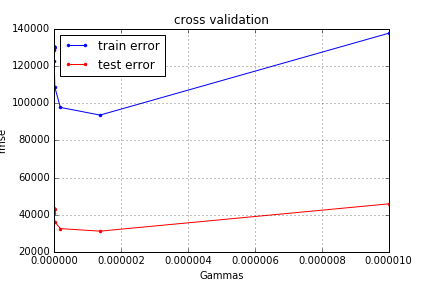
\includegraphics[width=3in]{figures/cross_validation_logistic}
    \caption{Cross validation for logistic regression}
    \label{fig:my_label}
\end{figure}


\section{Improvements of simple models}
\label{sec:tips-writing}
\subsection{Combined models}
To improve the predictions we started to combine different models together. The next step was to compute an initial
weight vector with a fast and efficient model like least squares or ridge regression and then start the logistic 
regression on theses weights. The difference of error wasn't significant and we didn't develop further with this method.

\subsection{Cross validation}
To validate (or invalidate) our models we use the cross validation technique to test them on the data. With this technique we also can find the best parameter lambda or gamma, depending on the methods, that minimize the loss.
We also compare different feature transformation (like polynomial basis).

This technique get a unbiased test error since the data are split into two subsets and the model is trained only on a sub-part of the initial data. Once the model has been trained, the remaining data that are not used for the training part are used to test the model. This gives an accurate unbiased test error.

\section{Final model choice}
Finally, after having tested the models above we selected the best one in order to have the best prediction.
As aforementioned, we used polynomial basis with degree 5; more precisely, here we also add a logarithm part due to efficient concern during testing state. Then we use a ridge regression on this data with a lambda value which has been optimized earlier with cross validation. With this lambda value, we could put further constrain to our learning method, avoiding model becomes too complex and thus cause the overfitting.
For this final model we also choose to ignore the features containing more than half unknown values because they also seems to be source of a biased prediction.
This had surely improve the prediction because the Higgs boson is a physical particle and observations is really important for such experiments so the quantity of observable states is certainly affecting the true state of the particle.

\section{Going further}

Possible ways to improve our result would be to do more pre-processing on the feature. By analyzing the data set, we could strengthen our learning method from the different importance of features and dealing better with low correlation data. 

I.e. the $22$th feature is canonical and has four possible values \(x \in \{0, 1, 2, 3\}\) 
which seems to be highly correlated to the output. The next step in order to improve our predictions would be to split the inputs and outputs into several data sets and train one model per data set. Each model would give a probability which belongs to one of the classification categories. In order to predict the category, we would split the input as well, compute the prediction and merge the data sets into one unique set. 

\end{document}

